\documentclass[t]{beamer}
\usepackage{pdfpages}
\usepackage{wrapfig}
\usepackage{cutwin}
\usetheme{Juelich}
\setbeamertemplate{footer element1}[logo]{arbor-lines-proto-colour}

\title{Introduction to Arbor}
\subtitle{What's new and demonstration}
\author{Brent F. B. Huisman}
\institute{Jülich Supercomputing Centre}
\date{\today}
\titlegraphic{\includegraphics%
    [width=\paperwidth]{placeholder}}

\newcommand{\lenitem}[2][.6\linewidth]{\parbox[t]{#1}{\strut #2\strut}}

\begin{document}
\maketitle

\small

\begin{frame}
    \frametitle{What is Arbor?}
    \framesubtitle{}
%     \vspace{0.5 \baselineskip}
        Arbor is a library for implementing performance portable network simulations of multi-compartment neuron models.
        % \begin{wrapfigure}{r}{20mm}
        %     \begin{center}
        %         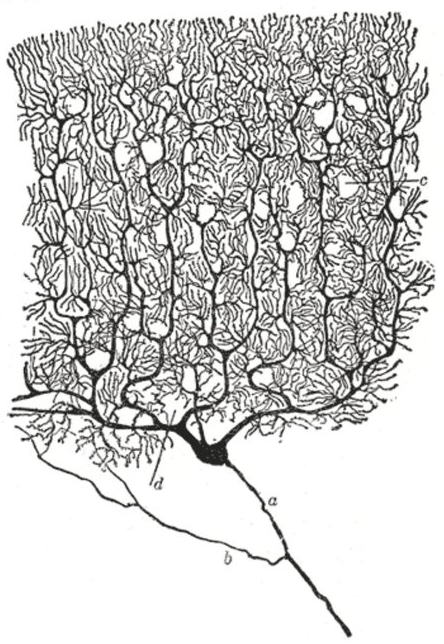
\includegraphics[width=\linewidth]{purkinje.png}
        %     \end{center}
        % \end{wrapfigure}

        \begin{itemize}
        \item Simulate large networks of morphologically-detailed, spiking neurons
        \item Library: you control your program/workflow. Interoperable.
        \item Portable: scientific description is separate from execution instructions. E.g. run one scientific description on laptop CPU, GPU cluster or future hardware.
        \item \textit{Performance} portable: add optimized backends for new computer architectures. Currently supported:
            \begin{itemize}
            \item Distributed parallelism using MPI
            \item CUDA backend for NVIDIA and AMD GPUs
            \item Vectorized backends for x86-64 (KNL, AVX, AVX2) and Arm64 (NEON, SVE) intrinsics
            \end{itemize}
        \item Executes on all HPC systems in the HBP (and outside).
        \end{itemize}
\end{frame}

\begin{frame}
    \frametitle{Who is Arbor?}
    % \framesubtitle{Cross-institutional effort}
    % \vspace{3\baselineskip}

    Open development style through Github
    \begin{itemize}
        \item Issues, PR workflow, Discussions, Slack/Gitter
        \item Code quality: PR review, unit testing, CI at Github and CSCS
    \end{itemize}

    \begin{wrapfigure}{r}{60mm}
        \begin{center}
            
\includegraphics[width=\linewidth]{cscs_logo.pdf}
        \end{center}
        \vspace{0.1\baselineskip}
        \begin{center}
            
\includegraphics[width=\linewidth]{Logo_FZJ_JSC.pdf}
        \end{center}
    \end{wrapfigure}

    Core contributors
    \begin{itemize}
        \item Ben Cumming
        \item Nora Abi Akar
        \item Stuart Yates
        \item Anne Küsters
        \item Thorsten Hater
        \item Brent Huisman
    \end{itemize}

    Website: \url{arbor-sim.org}

\end{frame}

{
\setbeamercolor{background canvas}{bg=}
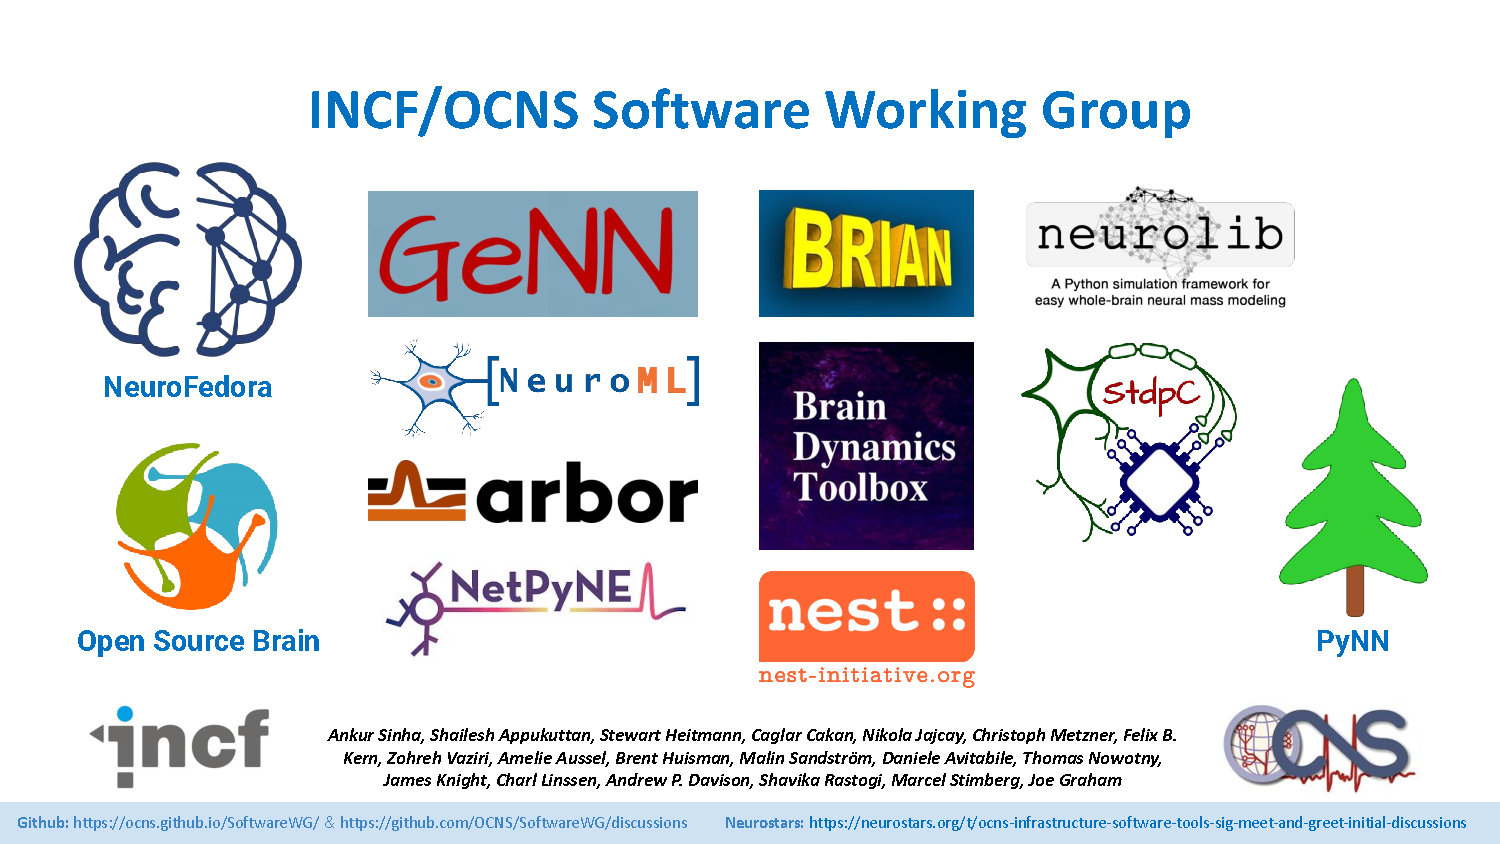
\includepdf[pages=1]{ocns-swg-slide.pdf}
}

\begin{frame}
    \frametitle{Arbor Status}
    % \framesubtitle{Some numbers}

    \begin{itemize}
        \item Latest release: v0.5.2
        \item 42 Github forks
        \item 1300+ commits to main branch
        \item loc: C++ header: 68k, C++: 68k, Python: 16k, reStructuredText: 8k
        \item 24 contributors, from 9+ institutions
        % from Lugano, Zürich, Jülich, Pavia, Oslo, Göttingen, Utrecht, Heidelberg, Barcelona, and more!
    \end{itemize}

    Ongoing collaborations:
    \begin{itemize}
    \item FIPPA - extend Arbor by key plasticity processes to simulate and analyze the long-term adaptive dynamics of large-scale, morphologically-detailed neuronal networks
    \item Arborio - large-scale model of the inferior olive of the cerebellar complex as a case study
    \item LFPy - investigating Arbor as possible backend
    \item Co-simulation - Nest, Elephant, TVB
    \end{itemize}

\end{frame}

%comp sci slide
\begin{frame}
    \frametitle{Building Arbor}
    \framesubtitle{begins with the computational model of neurons}

    \mbox{}\hfill\raisebox{-\height}[0pt][0pt]{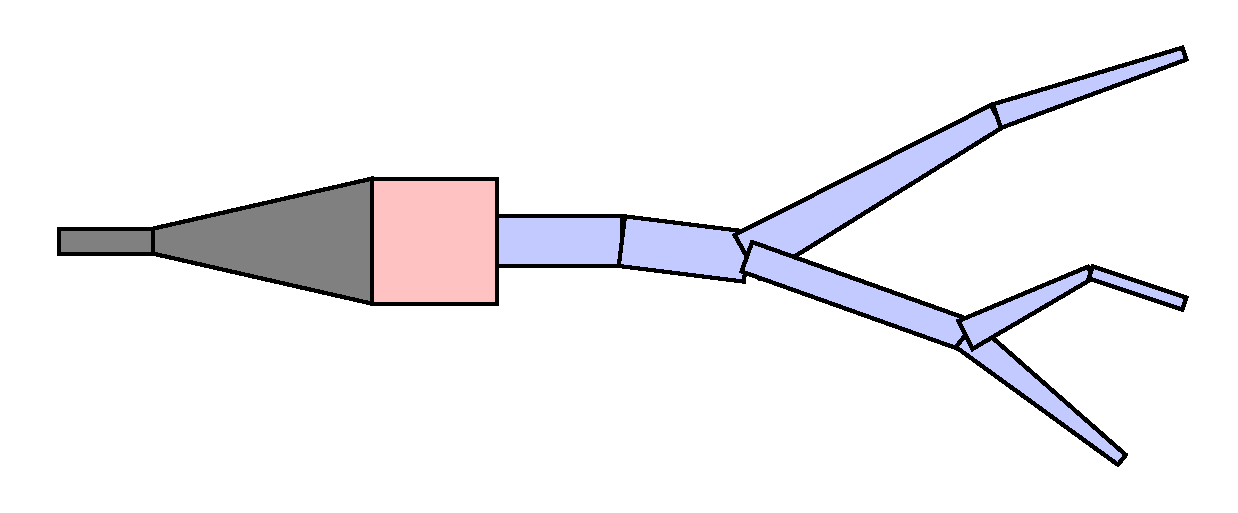
\includegraphics[width=.35\linewidth]{cell.pdf}}
    \vspace*{-\baselineskip}

    \begin{itemize}
    \item \lenitem{Arbor simulates networks of multi-compartment neurons}
    \item \lenitem{Neurons: approximated by axonal delay, synaptic functions and a set of cables connected in a tree.}
    \item Cables: characterized as electrical compartments (frustums) composed of ion channels, cable resistance and capacitance.
    \item Neurons represented as sparse, close-to-band matrices to be solved (e.g. by Hines solver) against known current states due to synaptic conductance.
    \item Network and spike exchange between neurons at synapses are represented by concatenations of matrices.
    \end{itemize}

\end{frame}

% \begin{frame}
%     \frametitle{Goals: interoperability}
%     \framesubtitle{Aiming for interoperability by being a simulator as library}
%     \begin{itemize}
%     \item Visualization with coupling to in-situ visualization and analysis tools
%     \item Multi-physics: can be integrated with other tools
%     \item Multi-scale from single neurons to large multi-compartmental networks
%     \item Usability: installable target and simple configuration, python front-end, efficient sampling of voltage and currents
%     \end{itemize}
% \end{frame}
%
% \begin{frame}
%     \frametitle{Goals: extensibility}
%     \framesubtitle{Aiming for extensibility by having modular internal API}
%     \begin{itemize}
%     \item New integration schemes, high-order time stepping, error control,
%     and efficient gap junction schemes
%     \item Custom spike communication and event systems,
%     \item API for receiving spikes live from external simulators (e.g. NEST)
%     \item Specialized cells: leaky integrate-and-fire, cable cell, Poisson spikes
%     \end{itemize}
% \end{frame}
%
% \begin{frame}
%     \frametitle{Goals: performance}
%     \framesubtitle{Aiming for high performance on HPC targets}
%     \begin{itemize}
%     \item Highly parallel and performance portable with task-based threading implementation, GPU and SIMD vector targets using NMODL and modcc
%     \item Design for scalability with fine-grained allocation of CPU and GPU resources
%     \item Reporting on memory and energy consumption
%     \item Unit testing, continuous integration, validation and a benchmarking suite (NSUITE)
%     \end{itemize}
% \end{frame}

% breakdown: mech, morph, network, am i missing sth?

\begin{frame}\footnotesize
    \frametitle{User design}
    \framesubtitle{Describe the neuroscience first ...}
\begin{columns}
    \begin{column}{0.45\textwidth}
    \begin{block}{Cells}
        \begin{itemize}
        \item Cells represent the smallest model to be simulated
        \item Cells are the smallest unit of work distributed across processes
        \item Types:
            \begin{itemize}\footnotesize
            \item Cable cells
            \item Leaky integrate-and-fire cells
            \item Spiking cells
            \item (Benchmark cells)
            \end{itemize}
        \end{itemize}
    \end{block}
    \end{column}
    \begin{column}{0.55\textwidth}
    \begin{block}{Recipes}
        \begin{itemize}
        \item Recipes describes models in a cell-oriented manner and supplies methods to:
            \begin{itemize}\footnotesize
            \item Map global cell identifier gid to cell type
            \item Describe cells (Cable cell 123, what is it's morphology?)
            \item List all connections from other cells that terminate on a cell
            \end{itemize}
        \item Advantage: parallel instantiation of cell data
        \end{itemize}
    \end{block}
    \end{column}
\end{columns}
\end{frame}

\begin{frame}\footnotesize
    \frametitle{User design}
    \framesubtitle{... then translate it into execution.}
\begin{columns}
    \begin{column}{0.45\textwidth}
    \begin{block}{Cell groups}
        \begin{itemize}
        \item Cell groups represent a collection of cells of the same type together with implementation of their simulation
        \item Partitioning into cell groups provided by decomposition
        \item A \textbf{simulation} manages instantiation of model and scheduling of spike exchange as well as integration for each cell group
        \end{itemize}
    \end{block}
    \end{column}
    \begin{column}{0.55\textwidth}
    \begin{block}{Mechanisms}
        \begin{itemize}
        \item In a recipe, mechanisms are specifications of ion channel and synapse dynamics. Advantage: parallel instantiation of cell data.
        \item[] Implementations of mechanisms:
        \item Hand-coded for CPU/GPU execution
        \item A translator (modcc) compiles a subset of NMODL to architecture-optimized vectorized C++ or CUDA
        \item Soon: Arblang
        \end{itemize}
    \end{block}
    \end{column}
\end{columns}
\end{frame}

% \begin{frame}\footnotesize
%     \frametitle{Arbor Design}
%     \framesubtitle{Summary}
%     Arbor models:
%     \begin{itemize}
%     \item Multicompartment neurons using a cable model transformed into a sparse matrix
%     \item Neurons characterized by axonal delays, synaptic functions and cables connected in a tree
%     \item Spike exchanges are global across computer nodes, functionally concatenating matrices
%     \end{itemize}

%     Models are composed of:
%     \begin{itemize}
%     \item Cells representing the small unit of computation (LIF, Artificial sources, Multicompartment cells)
%     \item Recipes representing a parallelizable set of neuron construction and connections
%     \item Cell groups computed together on the GPU or CPU
%     \item Mechanism representing ion channel and synapse dynamics
%     \end{itemize}
% \end{frame}

\begin{frame}
    \frametitle{Internal design}
    \framesubtitle{Programming interface ensures extensibility}
    \begin{center}
        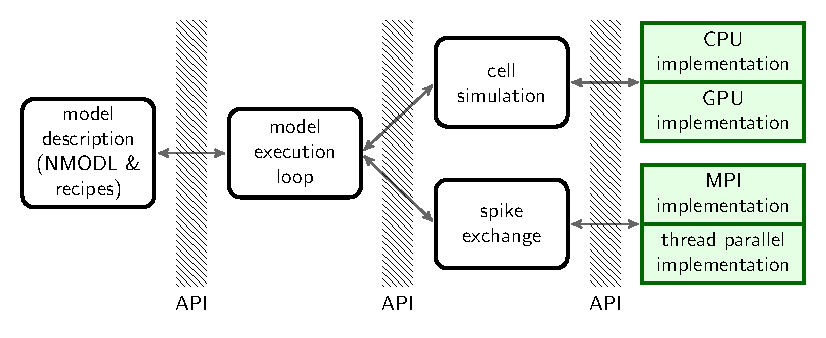
\includegraphics[width=0.9\linewidth]{api.pdf}
    \end{center}
    \begin{itemize}
    \item Components can be substituted according to the internal API.
    \end{itemize}
\end{frame}

% \begin{frame}
%     \frametitle{Internal design}
%     \framesubtitle{Computational work is hidden in backends}
%     \begin{center}
%         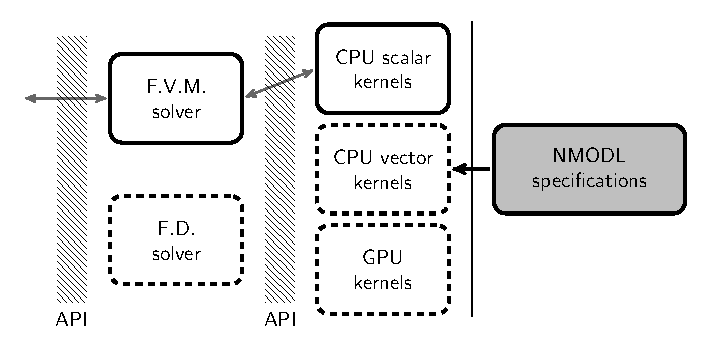
\includegraphics[width=0.7\linewidth]{backend-api.pdf}
%     \end{center}
%     \begin{itemize}
%     \item Cell simulation modules share computational backends for channel and synapse state evolution.
%     \item CPU-hosted finite volume cell simulation.
%     \end{itemize}
% \end{frame}

\begin{frame}
    \frametitle{Design}
    \framesubtitle{Summary}

    Arbor internal model:
    \begin{itemize}
    \item Internal API decouples model description, execution, spike exchange and cell simulation
    \item Computational work is hidden in pluggable backends, allowing automatic generation for different
architectures
    \end{itemize}

    User models are composed of:
    \begin{itemize}
    \item Cells representing the smallest unit of computation
    \item Recipes representing a parallelizable set of neuron construction and connections
    \item Mechanisms representing ion channel and synapse dynamics
%     \item Cell groups computed together on the GPU or CPU
    \end{itemize}
\end{frame}

\begin{frame}
    \frametitle{Interoperability, Portability and Extensibility}
    \framesubtitle{Why are they relevant to a computational neuroscientist?}
    \begin{itemize}
    \item Why a library?
    \begin{itemize}
    \item Makes Arbor interoperable with other tools and your way of working.
    \end{itemize}
    \item What is portability?
    \begin{itemize}
    \item Write your science and let Arbor worry about how to efficiently execute it.
    \end{itemize}
    \item What is performance portability?
    \begin{itemize}
    \item You can extend Arbor to take advantage of new hardware without having to modify your scientific description. Your scientific description will continue to work.
    \end{itemize}
    \end{itemize}
\end{frame}

\begin{frame}
    \frametitle{What's new?}
    % \framesubtitle{Aiming for high performance on HPC targets}
    \begin{itemize}
    \item Expanded set of tutorials
    \item CI significantly expanded
    \begin{itemize}
    \item Automated building of Python and Spack packages
    \item Soon: Ebrains CD
    \end{itemize}
    \item File format compatibility: cell morphologies
    \begin{itemize}
    \item SWC
    \item NeuroML
    \item Neurolucida ASCII
    \item Arbor Cable Cell
    \end{itemize}
    \item Arbor GUI
    \begin{itemize}
    \item Focussed on cell design, decoration
    \item Can run single cell model simulations
    \end{itemize}
    \end{itemize}
\end{frame}


\begin{frame}
    \frametitle{What's cooking?}
    % \framesubtitle{Aiming for high performance on HPC targets}
    \begin{itemize}
    \item Arbor mechanism description language (codename ARBLANG)
    \begin{itemize}
    \item Declarative
    \item Simple, extendable and maintainable
    \item Capable of performing powerful optimizations on the source code
    \item Make support in other simulators easy, make Arblang translatable to/from similar DSLs (eg: NEUROML/LEMS, NMODL, SBML)
    \end{itemize}
    \item Crack the nut of distributed gap junctions
    \begin{itemize}
    \item MSc will study Wave Relaxation method this summer
    \item Arborio is investigating \textit{multi-}GPU cell groups
    \end{itemize}
    \item Implement synaptic plasticity, synaptic scaling, and structural plasticity
    \begin{itemize}
    \item FIPPA
    \end{itemize}
    \item LFP estimation
    \begin{itemize}
    \item Arborio
    \end{itemize}
    \end{itemize}
\end{frame}

\begin{frame}
    \frametitle{Wrap up}
    \framesubtitle{Questions?}
    \begin{itemize}
        \item Web: \url{arbor-sim.org}
        \item Docs: \url{docs.arbor-sim.org}
        \item Community: \url{github.com/arbor-sim/arbor/discussions}
        \item[]
    \end{itemize}

    { \scriptsize Acknowledgements: This research has received funding from the European Unions
    Horizon 2020 Framework Programme for Research and
    Innovation under the Specific Grant Agreement No. 720270
    (Human Brain Project SGA1), Specific Grant Agreement No.
    785907 (Human Brain Project SGA2), and Specific Grant
    Agreement No. 945539 (Human Brain Project SGA3). }
    \newline
    \begin{figure}[h]
        \begin{center}
            
\includegraphics[width=0.2\linewidth]{ebrains_logo.png}
            \hspace{2em}
            
\includegraphics[width=0.4\linewidth]{HBP_logo.jpg}
        \end{center}
    \end{figure}
\end{frame}

\begin{frame}
    \frametitle{Demo time!}
    \begin{itemize}
    \item We'll be doing the network ring tutorial:
    \item[] \texttt{docs.arbor-sim.org/en/latest/tutorial/network\_ring.html}
    \item[]
    \item You can follow along locally
        \begin{itemize}
        \item \texttt{pip install arbor}
        \item Materials: \url{https://arbor-sim.org/ocns-2021/}
        \end{itemize}
    \item[]
    \item or connect at \url{https://jupyter-jsc.fz-juelich.de}
        \begin{itemize}
        \item Register here: \url{https://judoor.fz-juelich.de/register}
        \item Then request access: \url{https://judoor.fz-juelich.de/projects/join/training2120}
        \end{itemize}
    \end{itemize}
\end{frame}


\begin{frame}
    \frametitle{Create a new Jupyterlab}
    \framesubtitle{at the Jülich Supercomputing Centre}
    \begin{itemize}
    \item Version: JupyterLab
    \item System: Jusuf
    \item Account: your account
    \item Project: training2120
    \item Partition: LoginNode
    \item[] Start!
    \item Open Terminal
    \item \texttt{source /p/project/training2120/setup}
    \item \texttt{pip install --install-option='--mpi' arbor}
    \item[] Ready.
    \end{itemize}
\end{frame}

\begin{frame}
    \frametitle{Step 0}
    \begin{itemize}
    \item Documentation at \texttt{docs.arbor-sim.org}
        \begin{itemize}
        \item 'Concepts' for conceptual explanation
        \item Python and C++ sections detail the matching conceptual pages
        \end{itemize}
    \item Today's plan
        \begin{itemize}
        \item Make a cell
        \item Make a recipe
        \item Run
        \item Visualize results
        \end{itemize}
    \item Navigate to the \texttt{exercises} directory
    \item Open \texttt{network\_ring\_step1.py}
    \end{itemize}
\end{frame}

\begin{frame}
    \frametitle{Step 1}
    \framesubtitle{Make a cell}
    \begin{figure}[h]
        \begin{center}
            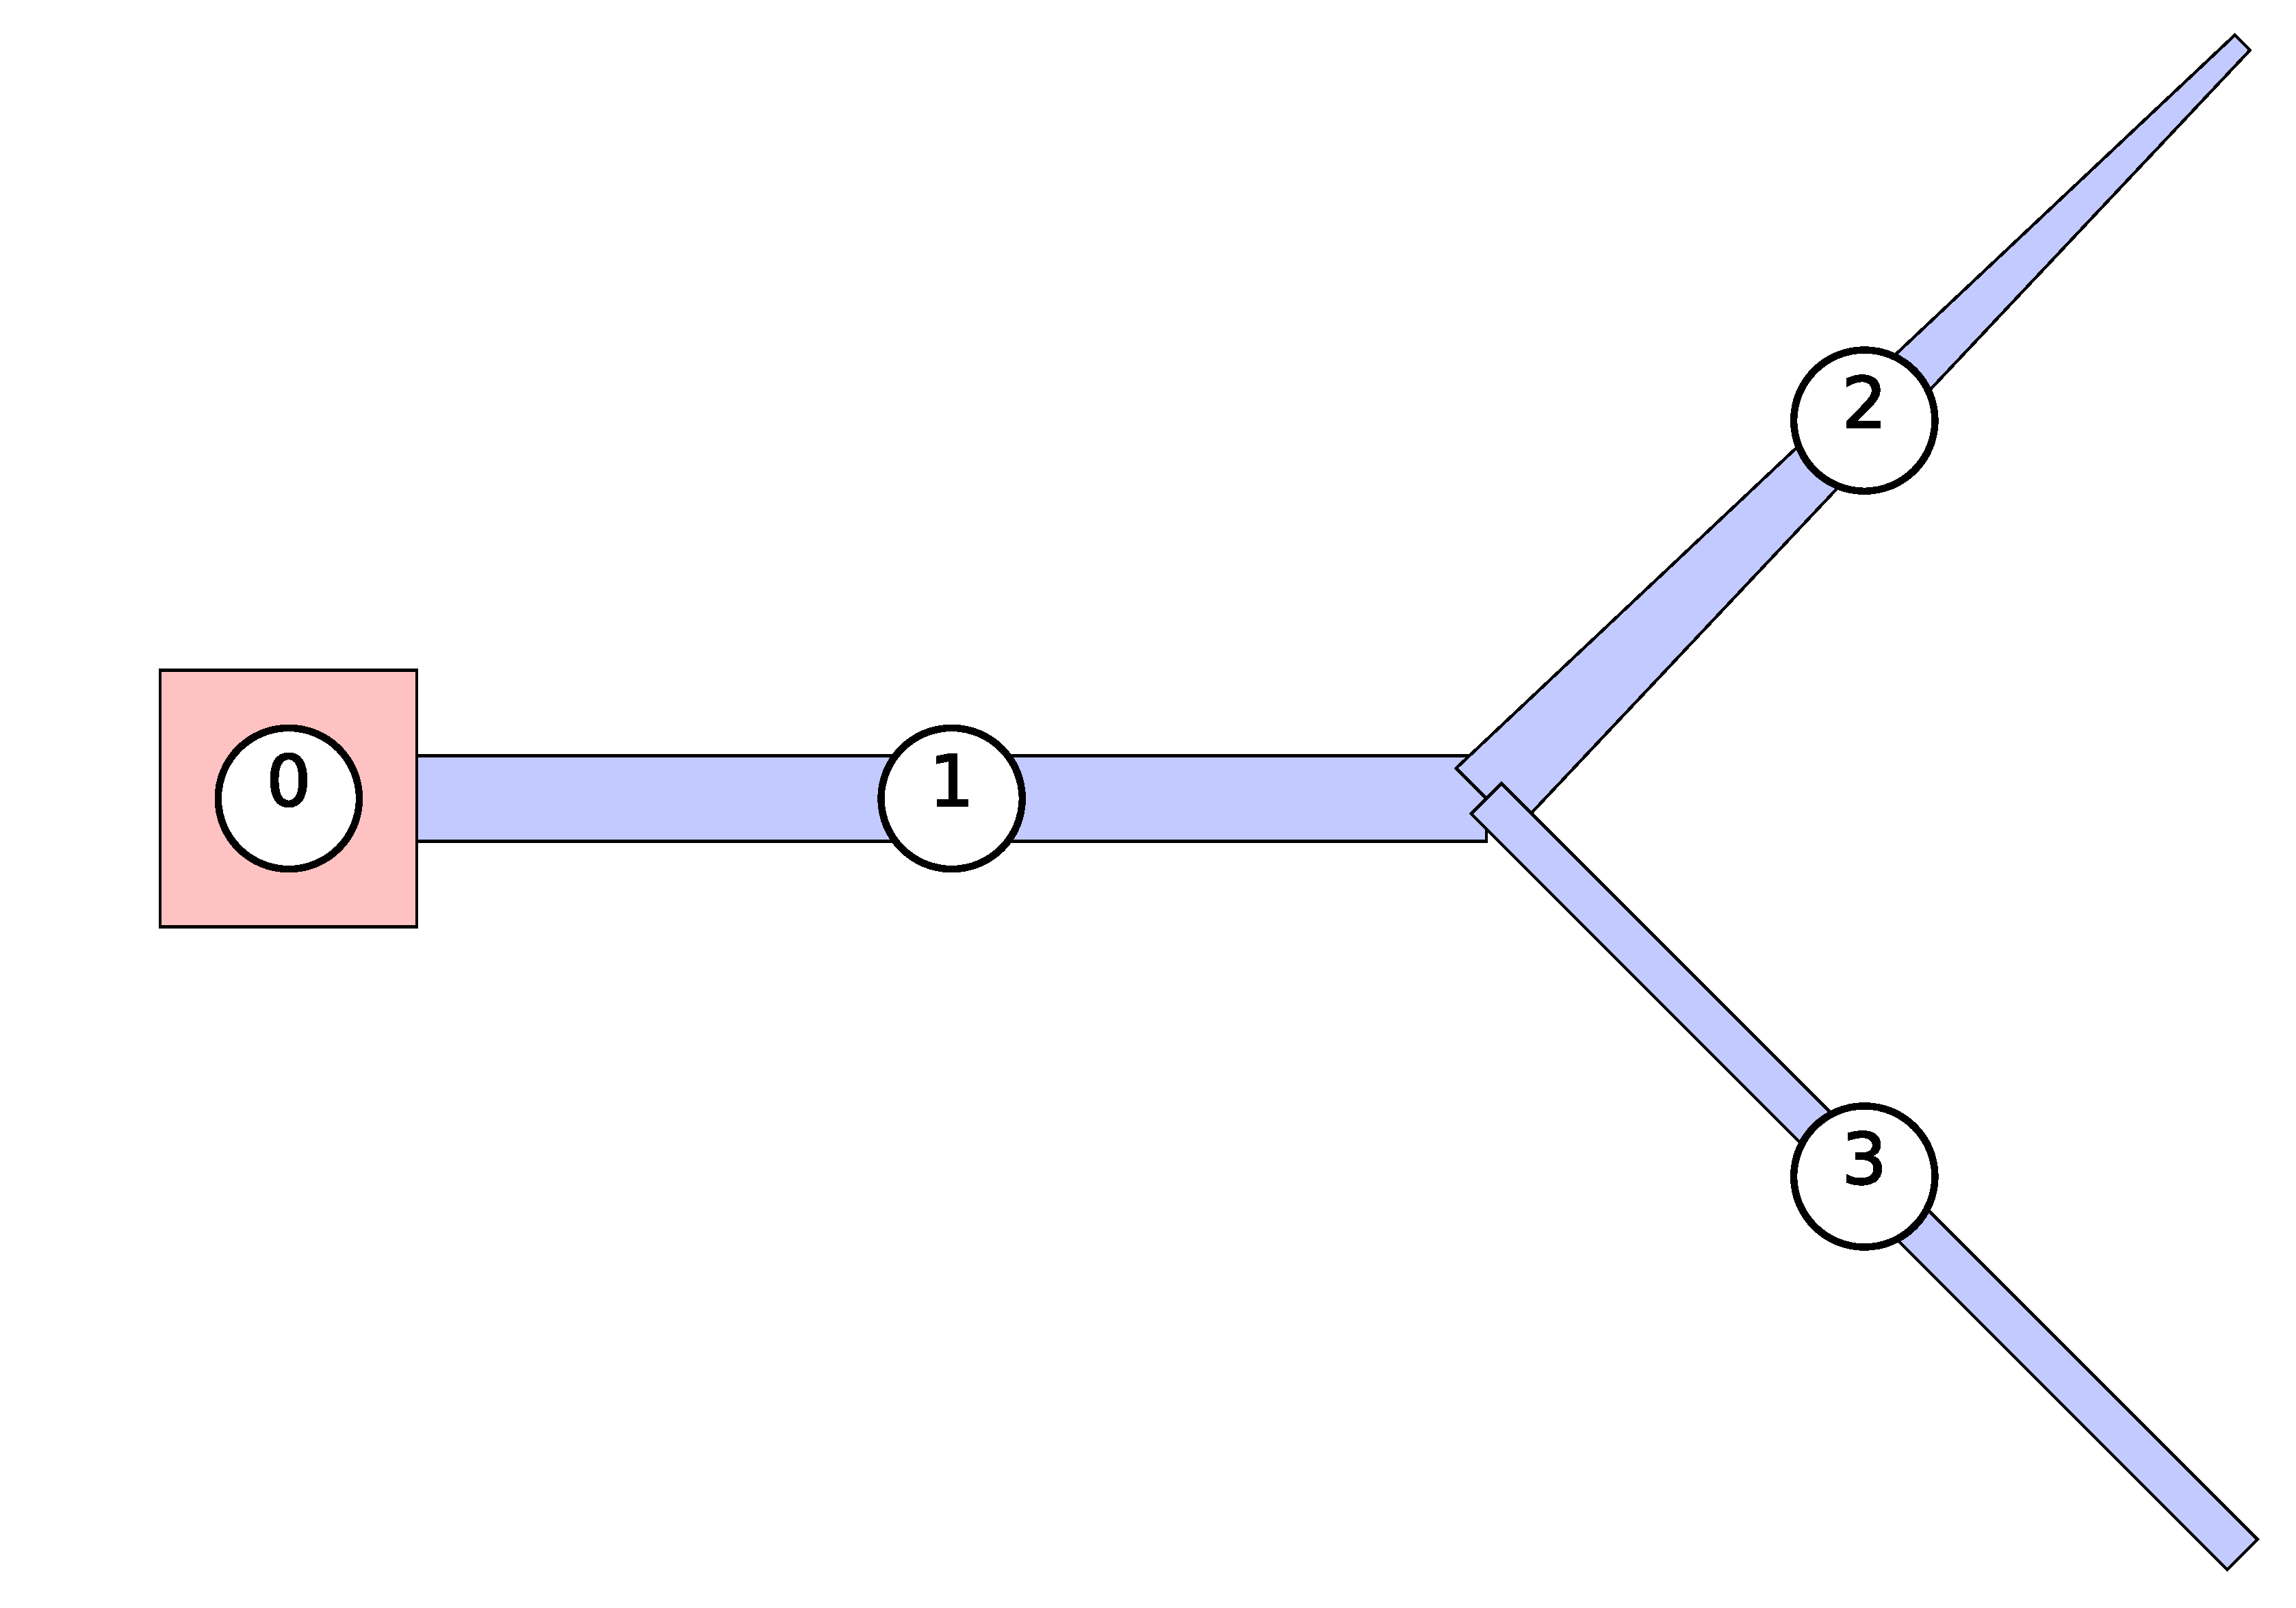
\includegraphics[width=0.45\linewidth]{tutorial_network_ring_morph}
            \hspace{2em}
            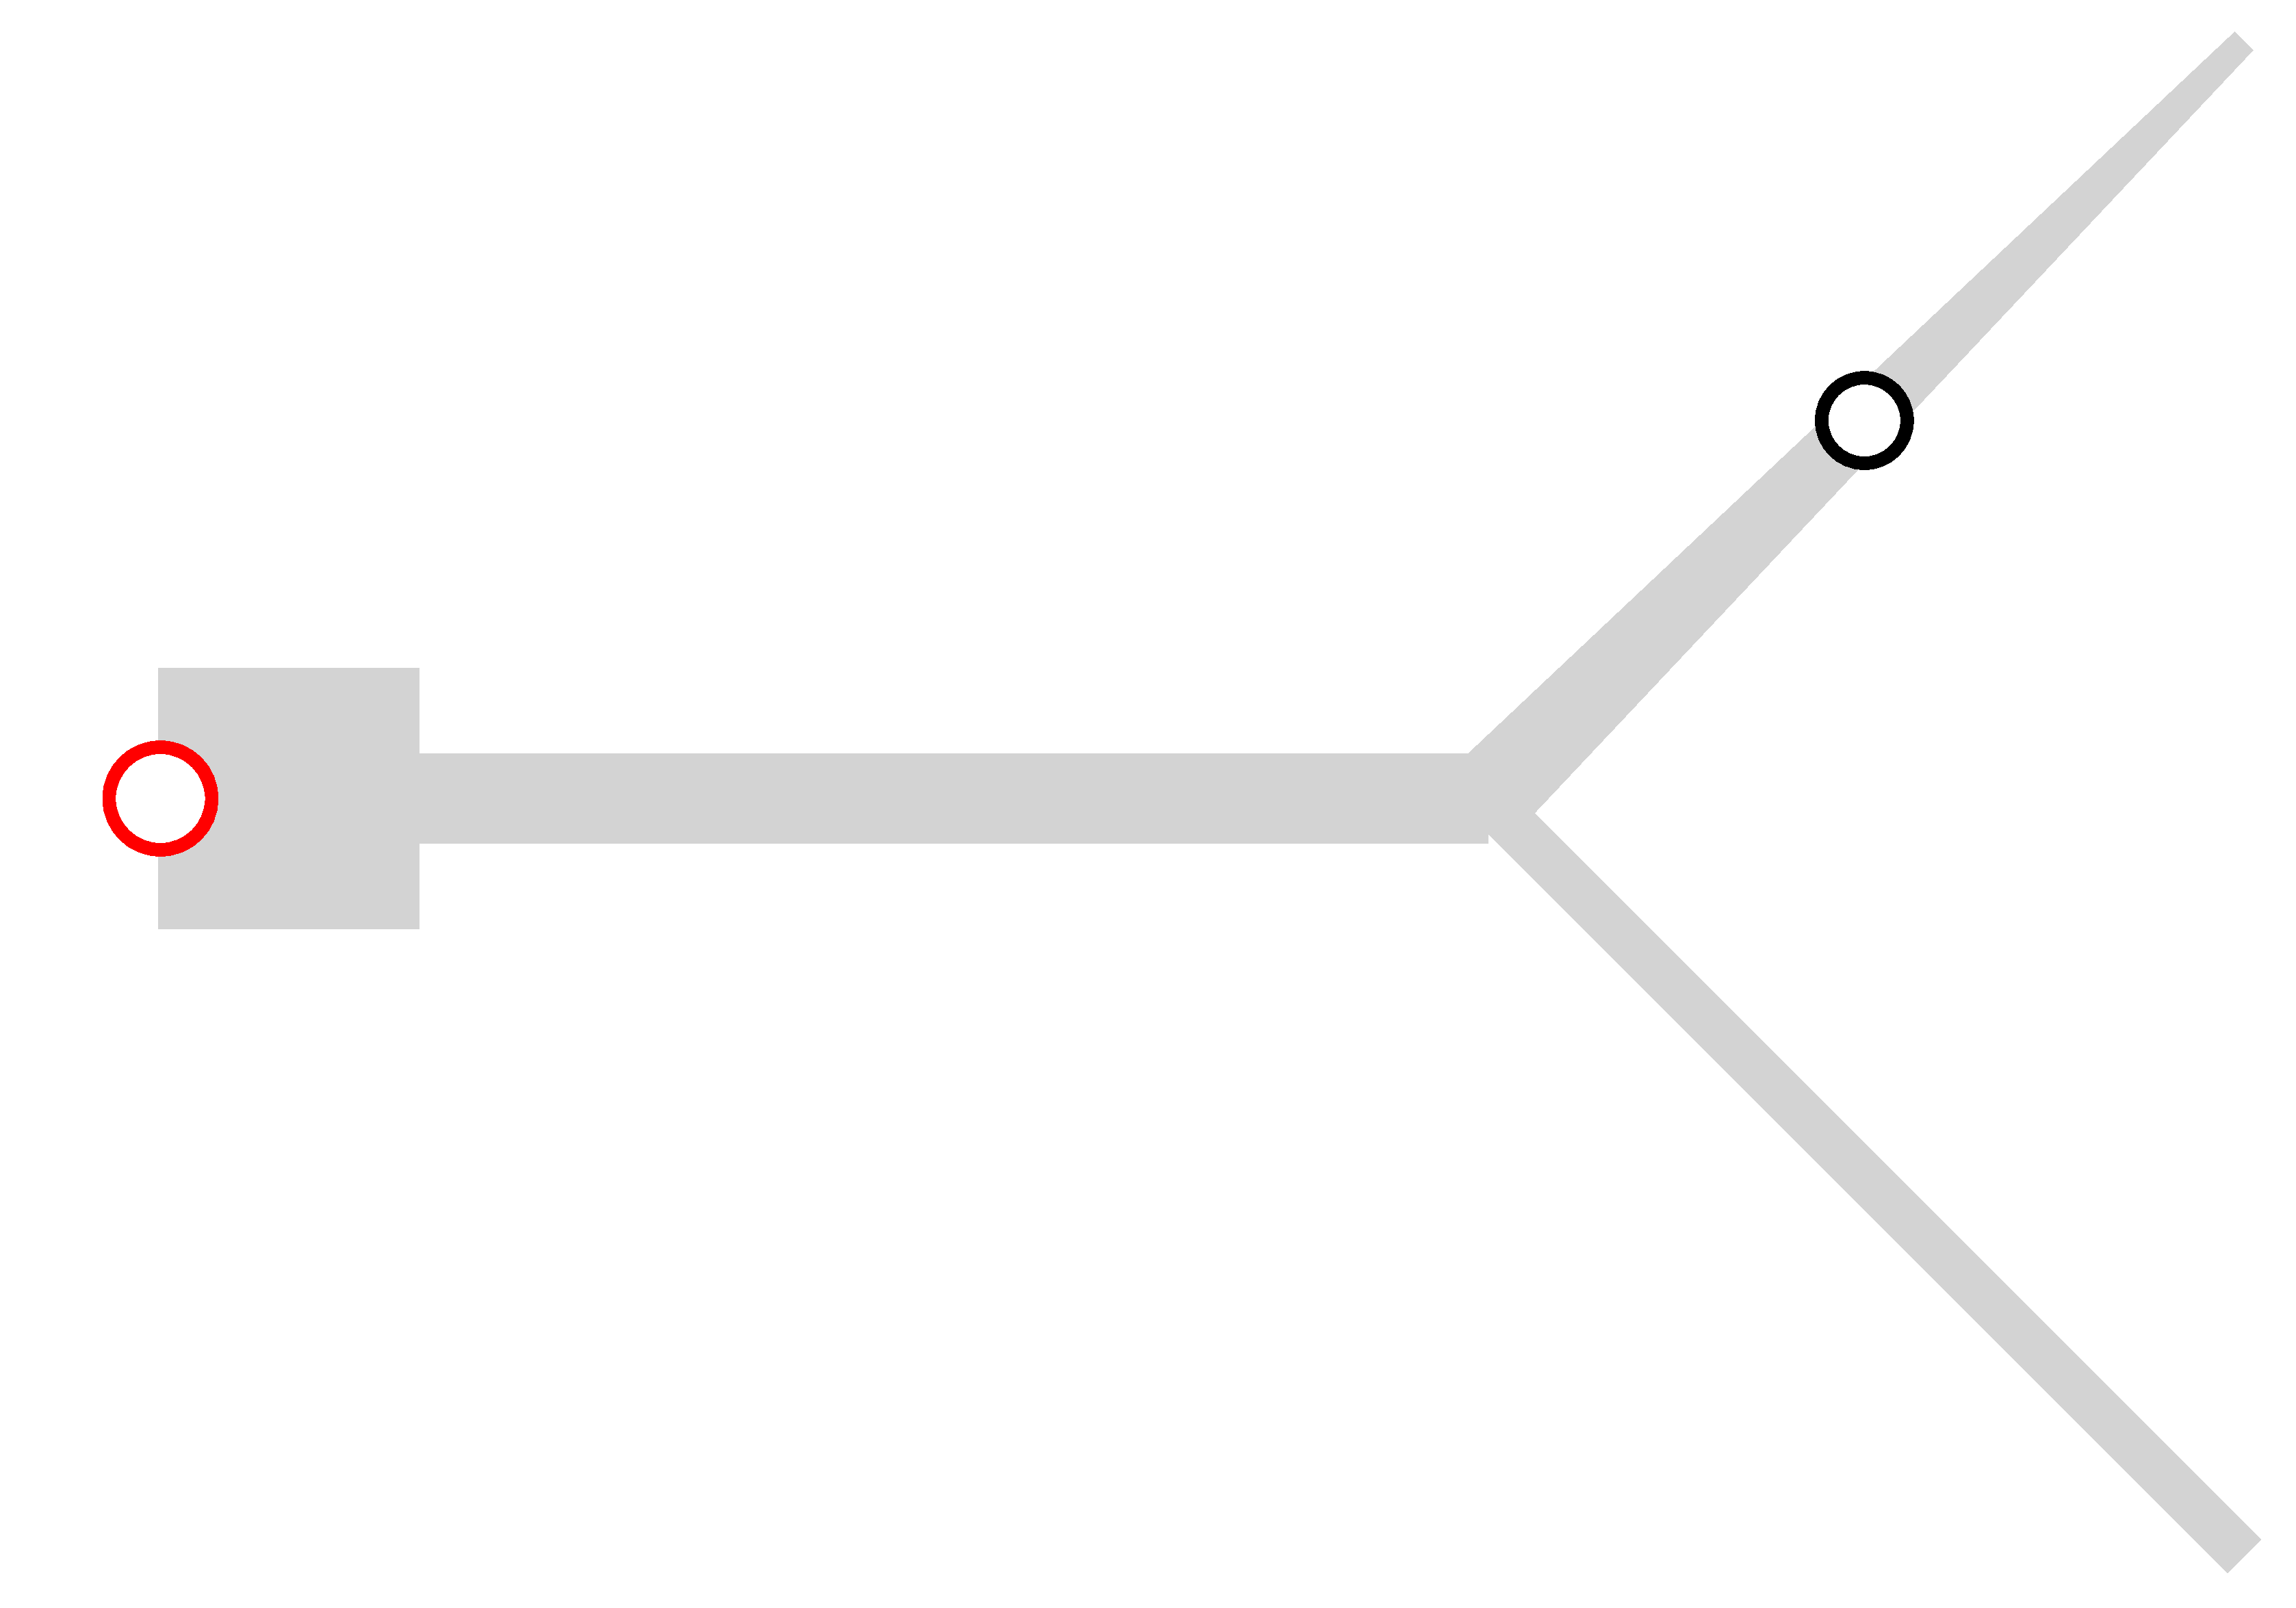
\includegraphics[width=0.45\linewidth]{tutorial_network_ring_synapse_site}
        \end{center}
        \caption{Left: Make a morphology of 4 segments: a soma (pink) and a branched dendrite (light blue). Right: We’ll create labels for the root (red) and a synapse\_site (black).}
    \end{figure}
\end{frame}


\begin{frame}
    \frametitle{Step 2}
    \framesubtitle{Make a network}
    \begin{itemize}
        \item Cells are the basic building blocks in Arbor
        \item Recipes tie them together
        \item You’ll make your own recipe by inheriting from \texttt{arbor.recipe}
        \item Some member functions need to be overridden
        \item Todo:
        \begin{itemize}
            \item Connect each cell with the previous
            \item Place an event generator on the first cell.
            \item Probe the membrane voltage at "root"
        \end{itemize}
    \end{itemize}
\end{frame}


\begin{frame}
    \frametitle{Step 3}
    \framesubtitle{Make a simulation}
    \begin{itemize}
        \item Describe
        \begin{enumerate}
            \item context (what hardware do you have?)
            \item domain decomposition (how to use the hardware)
            \item simulation
        \end{enumerate}
        \item Start with an \texttt{arbor.simulation} object, and see what you need for it.
        \item (defaults are OK)
        \item We need to store handles to the samplers, because later we’ll use \texttt{arbor.simulation.samples()} to retrieve results.
    \end{itemize}
\end{frame}


\begin{frame}
    \frametitle{Step 4}
    \framesubtitle{Show your results!}
    \begin{itemize}
        \item We can extract results from
        \begin{itemize}
            \item \texttt{arbor.simulation.spikes}
            \item \texttt{arbor.simulation.samples}
        \end{itemize}
        \item Print or plot
        \begin{itemize}
            \item I use Pandas and Seaborn
            \item \texttt{pip install pandas seaborn}
        \end{itemize}
    \end{itemize}
\end{frame}

\begin{frame}
    \frametitle{Bonus}
    \framesubtitle{Arbor on HPC}
    \begin{itemize}
        \item We’re going big! MPI!
        \begin{itemize}
            \item \url{https://en.wikipedia.org/wiki/Message\_Passing\_Interface}
        \end{itemize}
        \item Lookup \texttt{arbor.mpi\_comm} and how to use it.
        \item An \texttt{arbor.simulation} will now run distributed
        \begin{itemize}
            \item \texttt{arbor.simulation.samples} only knows about local results
            \item You’ll need to save results from the instances yourself!
        \end{itemize}
        \item \texttt{srun -A training2120 -n 5 python network\_ring\_mpi.py}
    \end{itemize}
\end{frame}


\begin{frame}
    \frametitle{The end}
    \framesubtitle{Questions?}
    \begin{itemize}
        \item Web: \texttt{arbor-sim.org}
        \item Docs: \texttt{docs.arbor-sim.org}
        \item Contact: \texttt{contact@arbor-sim.org}
        \item Community: \texttt{github.com/arbor-sim/arbor/discussions}
        \item[]
    \end{itemize}

    { \scriptsize Acknowledgements: This research has received funding from the European Unions
    Horizon 2020 Framework Programme for Research and
    Innovation under the Specific Grant Agreement No. 720270
    (Human Brain Project SGA1), Specific Grant Agreement No.
    785907 (Human Brain Project SGA2), and Specific Grant
    Agreement No. 945539 (Human Brain Project SGA3). }
    \newline
    \begin{figure}[h]
        \begin{center}
            
\includegraphics[width=0.2\linewidth]{ebrains_logo.png}
            \hspace{2em}
            
\includegraphics[width=0.4\linewidth]{HBP_logo.jpg}
        \end{center}
    \end{figure}
\end{frame}

\end{document}
